\documentclass[conference]{IEEEtran}
\IEEEoverridecommandlockouts
% The preceding line is only needed to identify funding in the first footnote. If that is unneeded, please comment it out.
\usepackage{cite}
\usepackage{amsmath,amssymb,amsfonts}
\usepackage{algorithmic}
\usepackage{graphicx}
\usepackage{textcomp}
\usepackage{xcolor}
\usepackage{url}
\def\BibTeX{{\rm B\kern-.05em{\sc i\kern-.025em b}\kern-.08em
    T\kern-.1667em\lower.7ex\hbox{E}\kern-.125emX}}

% ==== notation macros ==== 
\newcommand{\act}{\boldsymbol{a}}          % action trajectory
\newcommand{\ind}{\mathbf{1}}              % indicator
\newcommand{\Acal}{\mathcal{A}}            % action vocabulary
\newcommand{\Mcal}{\mathcal{M}}            % compatibility relation
\newcommand{\Ccal}{\mathcal{C}}            % motion-class set
\newcommand{\todo}[1]{\textcolor{red}{[TODO: #1]}}

\setlength{\textfloatsep}{6pt plus 2pt minus 2pt}
\setlength{\floatsep}{6pt plus 2pt minus 2pt}
\setlength{\intextsep}{6pt plus 2pt minus 2pt}
\setlength{\abovecaptionskip}{3pt}
\setlength{\belowcaptionskip}{2pt}

\setlength{\fboxsep}{2pt}
\begin{document}

\title{Action-Grounded VLM Reasoning for Autonomous Vehicle Semantic Anomalies\\
% {\footnotesize \textsuperscript{*}Note: Sub-titles are not captured in Xplore and should not be used}
% \thanks{Identify applicable funding agency here. If none, delete this.}
}

\author{\IEEEauthorblockN{Daniel Adejumo\textsuperscript{2}, Omkar Ankalkope\textsuperscript{2}, Kunal Runwal\textsuperscript{2}, and Aliasghar Arab\textsuperscript{1,2,$*$}}%
\thanks{\textsuperscript{1}Aliasghar Arab is with The City College of New York, Grove School of Engineering, New York, NY 10031, USA. aarab@ccny.cuny.edu}%
\thanks{\textsuperscript{2}Daniel, Omkar, Kunal and Aliasghar are with the Department of Mechanical and Aerospace Engineering, Tandon School of Engineering, New York University, 6 MetroTech Center, Brooklyn, NY 11201, USA (ASAS-Labs). aliasghar.arab@nyu.edu}%
% \thanks{\textsuperscript{$*$}Corresponding author.}%  <-- uncomment/adjust: the meaning of the asterisk was not specified
}

\maketitle

\begin{abstract}
Deployed autonomous vehicles (AVs) increasingly encounter \emph{semantic anomalies}: perception works as designed yet the vehicle behaves incorrectly because a familiar object appears outside its nominal context (a stop sign on a billboard, brake lights on a video screen, a fire hose across a live lane). Vision--language models (VLMs) are commonly applied to this problem with scene video and an ``is this anomalous?'' prompt. We show this formulation is inherently ambiguous: the anomaly is defined by the ego vehicle's \emph{response}, not the scene alone. We therefore propose action-grounded anomaly reasoning, in which the VLM receives the ego action sequence (velocity and heading over time) alongside the video. We introduce a six-field framework for generating semantic anomalies, a taxonomy of 112 scenario pairs spanning both failure polarities (42 grounded in documented incidents, including NHTSA recalls and NTSB investigations), and \textbf{av\_semantic\_anomalies}, the first action-grounded semantic-anomaly dataset for AVs: world-model-generated driving videos with per-timestep ego-action trajectories recovered via inverse dynamics, in matched normal/anomalous pairs for most scenarios. At inference, a two-stage protocol derives the scene-required action from an action-blind early window, then checks the vehicle's actual trajectory against it, improving accuracy from 74.5\% to 82.1\% and anomaly recall from 0.54 to 0.76 over the strongest video-only baseline.
\end{abstract}

\begin{IEEEkeywords}
semantic anomaly detection, autonomous vehicles, vision--language models, action grounding, runtime monitoring, world models
\end{IEEEkeywords}

\section{Introduction}\label{sec:intro}

Autonomous vehicles (AVs) now operate at commercial scale, and with that scale has come a steady record of failures in which perception performs exactly as designed and the vehicle still behaves incorrectly: a stop sign correctly detected, but printed on a billboard; brake lights correctly recognized, but part of an advertisement; flat road debris correctly classified, but actually a charged fire hose. These \emph{semantic anomalies}~\cite{b1} arise from objects appearing outside their nominal context. Documented incidents (robotaxis driving over deployed fire hoses, entering flooded roadways, passing stopped school buses, several ending in NHTSA recalls and NTSB investigations) show the failure class is a persistent obstacle to safe autonomy.

Early anomaly detection in driving operated on single images: OOD segmentation benchmarks (Fishyscapes~\cite{b2}, SegmentMeIfYouCan~\cite{b3}), generative resynthesis~\cite{b4}, corner-case detection (CODA~\cite{b5}), physical adversarial examples~\cite{b6}, and lately VLMs judging whether a frame is contextually unusual~\cite{b1}; but many semantic anomalies are defined by dynamics, invisible in a single frame. Video-based work supplies the temporal window: dashcam anomaly datasets (DoTA~\cite{b7}), language-aligned recognition (AnomalyCLIP~\cite{b8}), and driving-tuned multimodal models (DriveGPT4~\cite{b9}, DriveVLM~\cite{b10}, Cosmos-Reason1~\cite{b11}, post-trained by frameworks such as VLM-AutoDrive~\cite{b12}). The classic latency objection is closing: an NVFP4-quantized Cosmos-Reason1-7B reaches ${\sim}500$~ms per inference, a ${\sim}50\times$ speedup sufficient for continuous 1--2~Hz monitoring~\cite{b13}. Multi-view reasoning widens spatial context over standard surround rigs~\cite{b14}: BEV language maps~\cite{b15}, multi-view frameworks~\cite{b16}, spatio-temporal benchmarks~\cite{b17}, and view-grounding studies~\cite{b18} all report gains.

Yet even with full temporal and spatial context, one input remains missing: \emph{what the vehicle is doing}. The omission is definitional. A semantic anomaly is a property of the scene--action pair: the billboard stop sign is benign if the ego vehicle drives past and anomalous if it brakes; the fire-hose scene is handled correctly if the vehicle stops and catastrophically if it proceeds. ``Is there an anomaly?'' is thus ambiguous in principle (the same clip admits both labels depending on the ego response, for human annotators no less than VLMs), and without the ego action the model must guess the vehicle's behavior from subtle visual cues.

We close this gap by grounding VLM anomaly reasoning in the ego action: alongside the video, the model receives the vehicle's velocity-and-heading sequence and judges whether the \emph{behavior in context} reveals a semantic misunderstanding requiring intervention, converting an ill-posed scene-classification problem into a well-posed behavior-evaluation problem. No existing dataset can supervise this reframing: anomaly labels in dashcam corpora~\cite{b7}, corner-case sets~\cite{b5}, and driving QA benchmarks~\cite{b16,b17} attach to scenes or objects, not ego behavior, and standard perception suites~\cite{b14} contain almost no semantic-anomaly content. What is needed is a dataset in which each scenario appears with \emph{both} polarities of ego behavior, each paired with its action trajectory, so the label is unambiguous by construction.

We construct such a dataset. From a six-field generation framework (object, nominal context, OOD context, normal action, anomalous action, example scenario) we develop a taxonomy of 112 scenario pairs spanning both failure polarities, 42 grounded in documented incidents (NHTSA recalls, NTSB investigations, published adversarial-ML attacks), and release \textbf{av\_semantic\_anomalies}: world-model-generated ego-view videos in matched normal/anomalous pairs, each with a per-timestep action trajectory (velocity and heading at 5~Hz and 10~Hz) recovered via inverse dynamics and validated heuristically and manually.

Our contributions are threefold: (i) we identify and formalize the action-grounding gap, showing scene-only inference is inherently ambiguous; (ii) we propose action-grounded anomaly reasoning and demonstrate 74.5\% $\rightarrow$ 82.1\% accuracy with anomaly recall 0.54 $\rightarrow$ 0.76 over an otherwise identical video-only baseline; (iii) we release the framework, the 112-pair taxonomy, and the dataset. Section~\ref{sec:method} presents the methodology; Section~\ref{sec:results} the dataset, evaluation, and ablations; Section~\ref{sec:conclusion} concludes.

\section{Methodology}\label{sec:method}

\subsection{Semantic Anomalies Definition Framework}\label{sec:framework}

We define a \emph{semantic anomaly} as a driving failure in which perception performs as designed yet the vehicle behaves incorrectly because the object appears outside its nominal context~\cite{b1}: the detected stop sign \emph{is} a stop sign, but printed on a billboard, so the mandated response no longer applies. Semantic anomalies are disjoint from the pixel-level unknowns of OOD segmentation~\cite{b2,b3} (the object is in-distribution; its \emph{context} is not) and occupy the ISO~21448 (SOTIF) space of scenarios unsafe without any component fault~\cite{b19}.

To define such scenarios systematically we draw on hazard enumeration in safety engineering: HARA under ISO~26262~\cite{b20}, scenario-based testing~\cite{b21}, and recent LLM automation of these analyses~\cite{b22}, productized in platforms such as General Autonomy's G-Assess~\cite{b23}. Those methods enumerate hazards top-down from vehicle \emph{functions}; our framework instead factors the anomaly bottom-up around a driving entity and its context, and defines the label by the ego action within the scene.

Every scenario decomposes into the six fields of Table~\ref{tab:framework}, each field's output feeding the next. Fields 1--3 build the scene: a semantically loaded object with a mandated response, its nominal context, and a displacement of the object or a look-alike into an OOD context, appearance preserved, via reusable operators (\emph{relocate}, \emph{reprint}, \emph{carry as cargo}, \emph{reflect}, \emph{project}, \emph{natural mimic}). Fields 4--5 give the behavioral contrast: the Normal Action of a context-aware driver versus the Anomalous Action of a pattern-matching stack. Field 6 collapses the row into a one-sentence scenario used as the generation seed.

\begin{table}[htbp]
\caption{The six-field semantic-anomaly framework}
\begin{center}
\footnotesize
\begin{tabular}{|c|l|p{4.6cm}|}
\hline
\textbf{\#} & \textbf{Field} & \textbf{Description} \\
\hline
1 & Object in Driving Scene & Entity with a mandated response (stop sign, brake lights, pedestrian, fire hose) \\
\hline
2 & Nominal Context & Where the object normally lives; reacting to it there is correct \\
\hline
3 & OOD Context & Object or look-alike displaced outside its nominal context, appearance preserved \\
\hline
4 & Normal Action in OOD & Context-aware response: react to the scene, not the pattern \\
\hline
5 & Anomalous Action in OOD & Failure mode: react to the pattern as if nominal, or miss a real hazard presenting atypically \\
\hline
6 & Example Scenario & One-sentence description; the generation / evaluation prompt seed \\
\hline
\end{tabular}
\label{tab:framework}
\end{center}
\end{table}

Because fields 4--5 attach both behaviors to the same scene, every row yields a \emph{scenario pair}: two clips identical except for the ego action, one Normal, one Anomalous, the label unambiguous by construction. The pairing covers both polarities: \emph{false-positive} (FP) failures act on a non-threat (braking for the billboard sign); \emph{false-negative} (FN) failures ignore a disguised real threat (driving over a charged fire hose). Table~\ref{tab:examples} shows one instantiated row of each.

\begin{table*}[htbp]
\caption{Example scenario pairs, one per failure polarity}
\begin{center}
\footnotesize
\begin{tabular}{|p{1.4cm}|p{2.4cm}|p{2.7cm}|p{2.6cm}|p{2.5cm}|p{3.2cm}|c|}
\hline
\textbf{Object} & \textbf{Nominal Context} & \textbf{OOD Context} & \textbf{Normal Action} & \textbf{Anomalous Action} & \textbf{Example} & \textbf{Tag} \\
\hline
Fire hose & Coiled on a fire engine, off the roadway & Charged hose across an active lane at a fire scene & Stop before the hose; never cross; wait to be waved through & Classifies it as debris; drives over the hose & A car drives over a charged fire hose at an active fire scene & REAL $\cdot$ FN \\
\hline
Brake lights & Rear of a lead vehicle in the ego lane & Life-size car ad with glowing brake lamps on a night digital billboard & Recognize the screen as media; hold speed and lane & Reads a braking lead vehicle; brake-checks at speed & A car brake-checks for brake lights on a nighttime video billboard & SYN $\cdot$ FP \\
\hline
\end{tabular}
\label{tab:examples}
\end{center}
\end{table*}

Each row carries a provenance tag. \textbf{REAL} rows derive from documented incidents: the fire-hose row reproduces Cruise incidents at San Francisco fire scenes (2022--2023)~\cite{b24}; others include a Tesla repeatedly stopping for a Burger King logo~\cite{b25}, a taped ``35'' speed sign read as ``85''~\cite{b26}, a Waymo swept into a creek after entering a flooded roadway (a 3{,}791-vehicle recall)~\cite{b27}, and a Waymo passing a stopped school bus (an NTSB investigation)~\cite{b28}. Grounding in incidents that produced recalls and federal investigations targets failure modes with demonstrated safety impact.

\textbf{SYNTHETIC} rows extrapolate the same pattern to new object--context combinations, holding the framework logic fixed: the brake-lights row of Table~\ref{tab:examples} has no incident on record, but its mechanism class is documented (phantom responses to split-second signs on digital billboards~\cite{b29}), making it incident-adjacent rather than invented. The tabular form supports parallel authoring, completeness checking, and polarity balancing. The framework produced a 12-row seed taxonomy and a 100-row extension: 112 scenario pairs across ten categories, 42 REAL and 70 SYNTHETIC. \todo{REAL/SYNTHETIC tags for 12 rows pending; the count of 70 is tentative.} The ten categories are traffic-control-device look-alikes; pedestrian and humanoid confusions; animal anomalies; weather, smoke, and lighting; road surface and markings; unusual cargo and vehicles; emergency and event scenarios; adversarial and projected attacks; reflections and screens; and infrastructure, rail, and operational anomalies. Each row's Example field seeds the video generation of Section~\ref{sec:videogen}.

\subsection{Synthetic Video Generation}\label{sec:videogen}

Semantic anomalies are rare by construction, and no operator deliberately produces the \emph{anomalous} ego behavior, so balanced real footage is unobtainable. We instead synthesize the corpus with the Cosmos~3 world foundation model~\cite{b30}: each row's Example field, extended with the Normal or Anomalous action, seeds one ego-view video per polarity, the two clips depicting the same scene and differing only in the ego behavior. The pipeline comprises five stages.

\emph{(1) Prompt upsampling:} each sparse one-sentence seed is expanded by an LLM-based upsampler into a structured Cosmos~3 JSON prompt (subjects with counts, setting, lighting, cinematography, on-screen text, and a segmented action timeline), preserving the semantic core: object, OOD context, ego action. Because the label is carried by the ego action, each timeline is authored so the final, label-defining segment (the full stop before the hose, or the vehicle rolling over it) spans at least 2~s, with deceleration constrained to plausible windows (a smooth stop from cruising speed takes roughly 2.5--4~s), keeping the contrast resolvable for both inverse-dynamics recovery (Section~\ref{sec:action}) and the VLM. \emph{(2) Human validation of dense prompts:} a two-round realism review against a rubric (lighting, motion physics, geometry, traffic norms, object counts, cross-field contradictions); the \emph{intended} anomaly is exempt and must survive every edit. Round one corrects the sparse source and re-upsamples; round two fixes residuals in the JSON, every change logged, removing \emph{unintended} distribution shift while preserving the intended semantic shift.

\emph{(3) Scenery variation:} each validated prompt expands into roughly twenty variations (weather, lighting, time of day, urban context) preserving the semantic core, so each scenario polarity becomes a visually diverse clip family. \emph{(4) Video generation:} prompts are rendered by the Cosmos~3 text-to-video model served through a vLLM Omni stack, each yielding a 5-second (minority of scenes, 8-second), $832\times480$, 24~fps ego-view clip; generation used Cosmos3-Nano on one GPU (Cosmos3-Super is supported on a 4-GPU tensor-parallel configuration). \emph{(5) Human validation of generated videos:} each clip is reviewed against its source scenario for the intended object, OOD context, and ego action, plus artifacts and drift; feedback folds back into the sparse prompts and affected clips are regenerated. Passing clips constitute the paired videos of the dataset.

\subsection{Action Extraction from Synthetic Video Data}\label{sec:action}

Text-to-video generation produces pixels, not telemetry: we recover each clip's ego-action trajectory with the Cosmos~3 video-to-action inverse-dynamics pipeline, executed with Cosmos3-Nano.

Each 24~fps clip is first temporally resampled to 10~fps (7.5~fps for the 8~s clips) so the model's fixed 61-frame window spans the entire clip. The model predicts per-step translation and rotation (a 9-dimensional translation + 6D-rotation parameterization over the $T-1$ transitions); poses are composed, scaled to metric units, and reduced to two channels, ego \textbf{velocity} (mph) and \textbf{heading} (degrees, relative to the first frame), yielding a [velocity, heading] sequence at the resampled native rate (10~Hz; 7.5~Hz for 8~s clips) plus a 5~Hz downsample for token-constrained contexts. The channels mirror wheel-speed odometry and steering/yaw, transferring directly to production CAN signals without privileged simulator state.

Trajectories are validated twice: an automated heuristic compares each trajectory's tail against its prompt's label-defining final action (a prompted full stop should terminate near zero velocity; its anomalous twin should not), and a manual review in an interface playing the video beside synchronized velocity/heading plots records a Valid/Invalid judgment of realism and faithfulness. Failing clips are regenerated or excluded; regeneration is acceptance-gated, re-rendering under multiple seeds and accepting a candidate only when the recovered trajectory and an independent optical-flow motion probe both agree with the prompted action (68 clips of the release entered through this gate).

The output, paired clips with validated 5~Hz and 10~Hz trajectories, is the action grounding that Section~\ref{sec:vlm} supplies to the VLM.

\subsection{VLM Context and Anomaly Reasoning}\label{sec:vlm}

\begin{figure*}[!t]
\centering
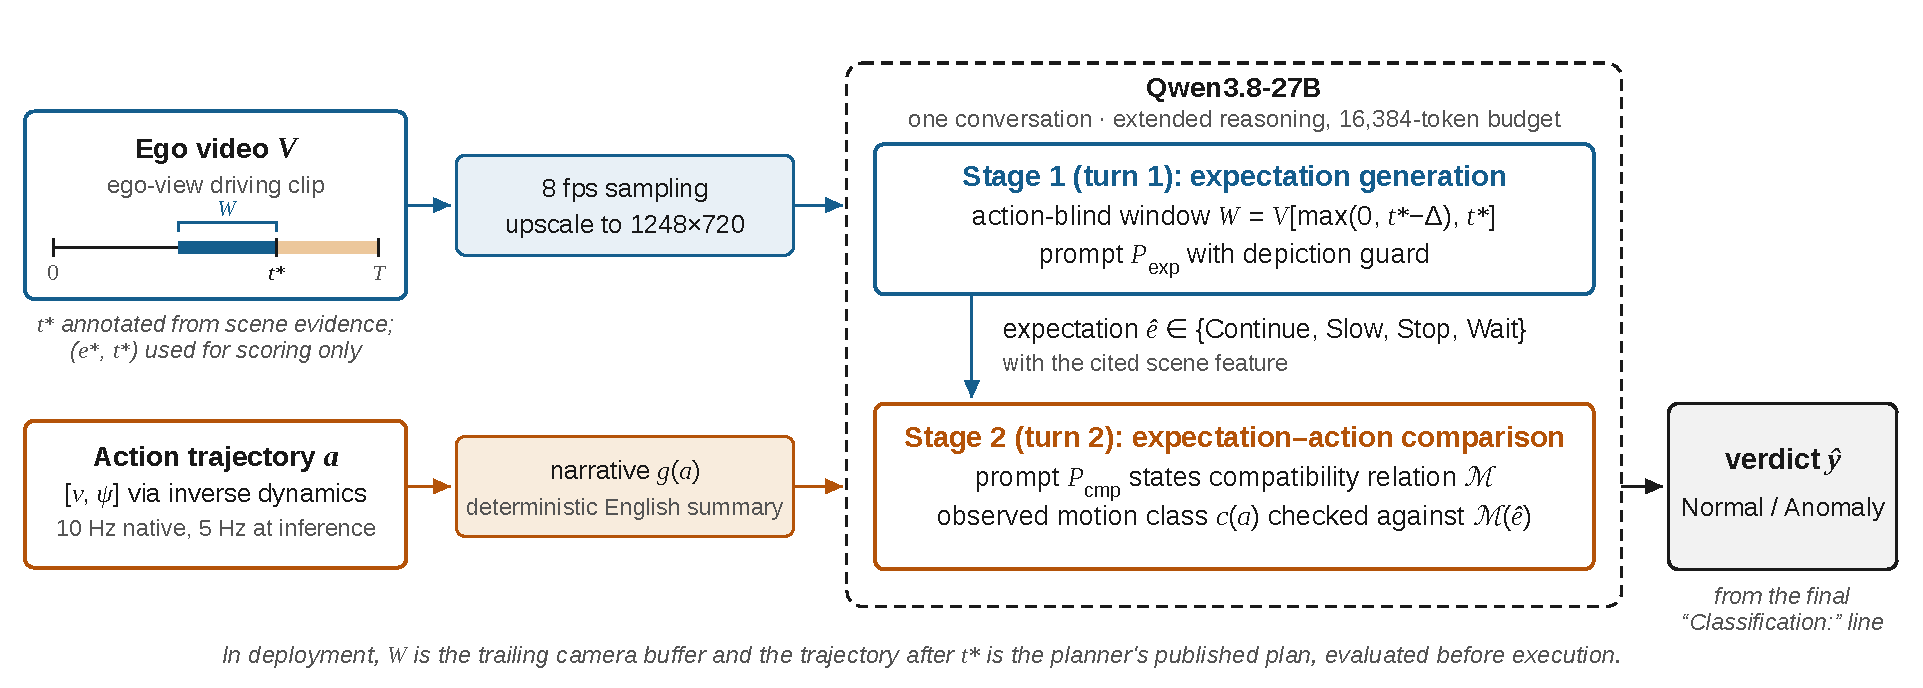
\includegraphics[width=\textwidth]{fig_pipeline_color.pdf}
\caption{The two-stage expectation--action anomaly monitor (video path in blue, action path in orange). Stage 1 sees only the action-blind window $W$ ending at the clip's decision time $t^*$ and produces the expected action $\hat{e}$; stage 2 compares the deterministic narrative rendering $g(\act)$ of the actual trajectory against the compatibility relation $\Mcal(\hat{e})$, yielding the verdict $\hat{y}$ of~\eqref{eq:label}.}
\label{fig:pipeline}
\end{figure*}

\paragraph{Problem formulation} Let $V$ denote an ego-view clip of duration $T$ and $\act = ((v_1, \psi_1), \dots, (v_K, \psi_K))$ its recovered trajectory (Section~\ref{sec:action}) at $f = 5$~Hz, $K = fT$. The prevailing formulation trains or prompts $h(V) \rightarrow \{\text{Normal}, \text{Anomaly}\}$, which Section~\ref{sec:intro} argued is ill-posed. We factor the judgment: with action vocabulary $\Acal = \{\text{Continue}, \text{Slow}, \text{Stop}, \text{Wait}\}$, let $e^* \in \Acal$ be the action a correct driver should take (framework field 4) and $c(\act) \in \Ccal = \{\text{continued}, \text{slowed}, \text{stopped}, \text{waited}, \text{moved off}\}$ the motion class the trajectory realizes. By construction,
\begin{equation}
y = \ind\!\left[\, c(\act) \notin \Mcal(e^*) \,\right],\label{eq:label}
\end{equation}
where $\Mcal : \Acal \rightarrow 2^{\Ccal}$ is a fixed compatibility relation (defined below). Equation~\eqref{eq:label} splits detection into two strictly simpler subproblems, \emph{expectation generation} and \emph{expectation--action comparison}, each one turn of a single VLM conversation (Fig.~\ref{fig:pipeline}), in the spirit of model-predictive runtime monitors~\cite{b31} with the ``should'' produced zero-shot from VLM world knowledge.

\paragraph{Model and serving} Both stages run zero-shot on Qwen3.8-27B~\cite{b32}, an open-weight VLM with native video input and extended reasoning~\cite{b33}, selected over the driving-tuned alternative of~\cite{b11} and five other open VLMs (Section~\ref{sec:ablations}); serving is vLLM~\cite{b34} with reasoning parser, 32{,}768-token context, fixed seed, and identical decoding for both stages (temperature 1.0, top-$p$ 0.95, top-$k$ 20, 16{,}384-token budget).

\paragraph{Input preprocessing} Video is sampled at 8~fps and upscaled from the native $832\times480$ to $1248\times720$ (Lanczos). Upscaling adds no information; its effect is architectural: the encoder allocates visual tokens by pixel area ($2.25\times$ more pixels, in practice ${\approx}\,1.5\times$ more tokens under the processor's pixel budget), so details below one patch at 480p survive patchification. This change is among the largest accuracy levers we found (Section~\ref{sec:ablations}); a 2.5~s window encodes to ${\approx}\,8.8$k visual tokens. The context is the single forward view; multi-view extensions~\cite{b15,b16,b17,b18} are orthogonal.

\paragraph{Stage 1: expectation from an action-blind window} The first turn supplies only an early video window
\begin{equation}
W = V\big[\max(0,\; t^* - \Delta),\; t^*\big], \qquad \Delta = 2.5~\mathrm{s},\label{eq:window}
\end{equation}
together with the expectation prompt $P_{\mathrm{exp}}$ of Fig.~\ref{fig:prompts}, eliciting $\hat{e} \in \Acal$: what a correct driver \emph{should} do next, plus the real scene feature requiring it. Two choices carry the weight. First, the window ends at the clip's \emph{decision time} $t^*$, the earliest instant at which the correct action is determinable from the scene (default $T - 2.5$~s; annotated per clip, from scene evidence only, where the hazard develops later); the pair $(e^*, t^*)$ is used only for scoring, never in prompts. Ending at $t^*$ keeps stage 1 blind to the label-defining behavior: with the full clip exposed, the ``expectation'' anchors on the visible ego action (a braking vehicle induces \emph{Stop}, which trivially matches), re-creating the ambiguity of~\eqref{eq:label}. Second, $P_{\mathrm{exp}}$ embeds a \emph{depiction guard}: an apparent traffic control or hazard that is only an image (printed, painted, displayed, reflected, worn, or carried) commands nothing; this sentence supplies the contextual rule defining the anomaly class (Section~\ref{sec:ablations}).

\paragraph{Stage 2: comparison against the actual action} The second turn supplies the full-clip trajectory $\act$ and the comparison prompt $P_{\mathrm{cmp}}$ of Fig.~\ref{fig:prompts}. Rather than raw numbers, the trajectory is rendered by a deterministic \emph{mechanical narrative} $g(\act)$: with $\bar{v}_0$, $\bar{v}_1$ the means of the first and last three speed samples, the renderer emits exactly one clause, \emph{moved off} ($\bar{v}_0 \leq 2$~mph $\wedge$ $\bar{v}_1 \geq 5$~mph), \emph{stopped} ($v_K \leq 2$~mph $\wedge$ $\bar{v}_0 > 5$~mph), \emph{slowed} ($\bar{v}_1 \leq 0.6\,\bar{v}_0$), \emph{sped up} ($\bar{v}_1 \geq 1.4\,\bar{v}_0$), else \emph{held steady}, with quantities inlined and a heading clause when $\max_k |\psi_k| \geq 10^{\circ}$. Pure arithmetic over the same numbers, $g$ leaks nothing beyond the trajectory; it removes the numeric-reading step, a known LLM failure surface~\cite{b35,b36}: given a correct expectation the comparator is essentially perfect with the narrative but errs on 17--30\% of clips with the raw $[[v, \psi], \dots]$ list (Section~\ref{sec:ablations}). $P_{\mathrm{cmp}}$ also states $\Mcal$ explicitly: \emph{continue} and \emph{slow} are mutually compatible, an expected \emph{stop} is satisfied by coming to rest or remaining at rest, the residual combinations are mismatches. The model states the observed motion class, compares, and emits $\hat{y}$ on its final line.

\paragraph{Reasoning mode and parsing} Both stages emit a delimited reasoning trace before the answer~\cite{b33,b37}; disabling reasoning loses 8--12 accuracy points, concentrated in the depiction traps (Section~\ref{sec:ablations}). The parser separates trace from answer, and only the answer decides: stage 1 is the option word on the final non-empty line, stage 2 the \emph{last} ``Classification:'' match, with deliberately no keyword fallback (traces rehearse both labels). Outputs with no parseable decision, including budget truncations, are scored incorrect (never resampled or extended), so parsing failures can only hurt; all raw outputs are retained. In the final configuration: zero truncations, $<1\%$ Unknown.

\begin{figure*}[htbp]
\centering
\fbox{\begin{minipage}{\dimexpr\textwidth-2\fboxsep-2\fboxrule\relax}\footnotesize
\textbf{System prompt:} ``You are a helpful assistant.''

\smallskip
\textbf{Stage 1 ($P_{\mathrm{exp}}$), with the early window $W$ attached:} ``You are evaluating the driving scene in this clip from the ego vehicle's point of view. Based only on what the scene requires---not on how the ego vehicle happens to be moving---what SHOULD a correct, safe driver do over the next few seconds? Name the specific real feature of the scene that requires it, or state that nothing requires a change. Note: an apparent traffic control or hazard that is only an image---printed, painted, displayed on a screen, reflected, worn on clothing, or carried as cargo---commands nothing. Then reply on the final line with exactly one word: Continue, Slow, Stop, or Wait. [the four options, each with a one-line gloss]''

\smallskip
\textbf{Stage 2 ($P_{\mathrm{cmp}}$), second turn of the same conversation:} ``Measured from the ego vehicle's own motion sensors over the recorded $\{T\}$ seconds of this clip: $\{g(\act)\}$. Read that motion as exactly one of: continued (speed roughly held), slowed (speed clearly reduced but still moving at the end), stopped (came to rest and stayed there), waited (stationary throughout), or moved off (pulled away from a standstill). Compare it with the expectation you gave. The behaviour MATCHES the expectation only for the action that was expected, with two tolerances: `continue' and `slow' are compatible with each other, and an expected `stop' is satisfied by coming to rest or remaining at rest. Stopping when continue or slow was expected, continuing or merely slowing when stop was expected, and moving off when wait was expected are mismatches. First state the observed motion class in one short sentence. Then reply on the final line with exactly one of: Classification: Anomaly---the behaviour does not match the expected action / Classification: Normal---the behaviour matches the expected action.''
\end{minipage}}
\caption{The two prompts of the expectation--action protocol, verbatim.}
\label{fig:prompts}
\end{figure*}

\paragraph{Deployment correspondence} On a vehicle, stage 1's window is the trailing 2.5~s camera buffer, re-evaluated continuously; $t^*$ of~\eqref{eq:window} is the step at which the monitor first has sufficient evidence. Stage 2's trajectory decomposes at $t^*$: recorded history before it, and after it the \emph{planned} trajectory the autopilot stack publishes for the next ${\approx}\,2.5$~s. The deployed monitor feeds stage 2 the concatenation of recorded history and planned horizon; our offline evaluation supplies exactly this object, the realized post-$t^*$ motion standing in for the plan. A mismatch (the plan brakes for a printed sign, or fails to brake for a charged hose) is flagged \emph{before execution}, in time to gate the plan or trigger a fail-safe handoff~\cite{b13,b31}.

\section{Results}\label{sec:results}

\subsection{Dataset}\label{sec:dataset}

The pipeline's primary artifact is \textbf{av\_semantic\_anomalies}, released openly on Hugging Face.\footnote{\url{https://huggingface.co/datasets/ASASLab/av_semantic_anomalies}} The taxonomy (112 pairs, ten categories, both polarities, REAL/SYNTHETIC 42/70) seeds the corpus; the current release instantiates the 12-row seed taxonomy as scenery-varied clip families (Section~\ref{sec:videogen}), most families in both polarities, each pair depicting the same scene under the correct and the incorrect ego action. \todo{instantiate the 100-row extension before publication and update the corpus figures.}

Each clip is 24~fps, $832\times480$ (480p), 5~s long (21 clips: 8~s), ego view without audio, generated with Cosmos3-Nano, and ships with two validated action files: the native-rate [velocity (mph), heading (deg)] sequence at 10~Hz (7.5~Hz for the 8~s clips) and a 5~Hz downsample that halves the token footprint for VLM inference, heading relative to the first frame. In total the release (\texttt{ASASLab/av\_semantic\_anomalies}) comprises 315 videos with 630 trajectory files, 1.09~GB.

Videos sit in a scenario-keyed tree with trajectories under the clip stem (\texttt{<stem>.txt} at 5~Hz, \texttt{<stem>\_10fps.txt} at 10~Hz; 8~s clips carry \texttt{<stem>\_7.5fps.txt}), so pairing is recoverable by filename alone. Provenance (REAL/SYNTHETIC), polarity (FP/FN), and the label are inherited from the seeding taxonomy row, supporting polarity- and provenance-stratified analyses.

\subsection{VLM Performance Evaluation}\label{sec:eval}

\paragraph{Evaluation subset} All results use a 235-clip subset (110 Anomalous / 125 Normal; 15 scenarios, both polarities) admitted by a three-witness agreement filter: the recovered trajectory must realize the prompted action (Section~\ref{sec:action}), an independent optical-flow probe must not contradict it, and the clip must pass human review; measured errors are thus the model's, not label noise. The majority-class baseline is 0.532.

\paragraph{Protocol} Inference follows Section~\ref{sec:vlm}: decision-time windows, 16{,}384-token reasoning budget, fixed seed, one clip per conversation. We report accuracy with 95\% Wilson intervals, balanced accuracy, recall (Anomalous), and specificity (Normal); unparseable or truncated outputs count as errors; paired comparisons use the two-sided exact McNemar test. Qwen3.8-27B was selected via the seven-model comparison of Table~\ref{tab:models}. All runs use one NVIDIA H200 (141~GB), bf16, request concurrency 6.

\paragraph{Results} Table~\ref{tab:monitor} reports the monitor with decision-time windows and with uniform fixed-lag $T-2.5$~s windows (differing on 25 clips): accuracy 0.821--0.830, balanced accuracy within a point, recall 0.76--0.77 at specificity 0.87--0.88, zero truncations and zero Unknown verdicts across all 470 stage calls. Errors localize sharply: the stage-2 comparator is correct on 180 of the 181 clips whose expectation is acceptable (99.4\%), so residual error is essentially all expectation generation ($181/235 = 77.0\%$ lenient-correct).

\paragraph{Comparison with the single-stage video-only baseline} Table~\ref{tab:monitor} compares against the strongest single-stage configuration found (Section~\ref{sec:ablations}): same model, budget, decoding, and depiction-guard concept, but one turn, video only, direct verdict, i.e., the prevailing formulation minus only action grounding and the two-stage factorization. It reaches 0.745 at a skewed operating point (specificity 0.928, recall 0.536), missing nearly half the anomalous behaviors by defaulting to Normal whenever the scene underdetermines the verdict, precisely the ambiguity of~\eqref{eq:label}. Action grounding lifts recall by 23 points at a 6-point specificity cost: +18 net clips (44 corrected vs 26 newly wrong; McNemar $p = 0.041$) and +8.6 points of balanced accuracy. Fig.~\ref{fig:example} shows the protocol end-to-end on an anomalous billboard clip.

\begin{table*}[htbp]
\caption{Two-stage expectation--action monitor vs. single-stage video-only baseline on the 235-clip evaluation subset (same model, budget, and guard; paired)}
\begin{center}
\footnotesize
\begin{tabular}{|l|c|c|c|c|c|c|}
\hline
\textbf{Method} & \textbf{Acc.} & \textbf{95\% CI} & \textbf{Bal. acc.} & \textbf{Recall} & \textbf{Spec.} & \textbf{Median latency} \\
\hline
Single-stage video-only (reasoning) & 0.745 (175/235) & [0.685, 0.796] & 0.732 & 0.536 & 0.928 & 61.8~s \\
\hline
\textbf{Two-stage action-grounded (ours), decision-time windows} & \textbf{0.821} (193/235) & [0.767, 0.865] & \textbf{0.818} & \textbf{0.764} & 0.872 & \textbf{46.9~s} \\
\hline
Two-stage, fixed-lag $T-2.5$~s windows & 0.830 & [0.777, 0.872] & 0.826 & 0.773 & 0.880 & -- \\
\hline
Majority class & 0.532 & -- & 0.500 & 0.000 & 1.000 & -- \\
\hline
Paired difference (ours vs. single-stage) & \multicolumn{2}{c|}{+18 net (44/26), McNemar $p = 0.041$} & +0.086 & +0.228 & $-0.056$ & $-14.9$~s \\
\hline
\end{tabular}
\label{tab:monitor}
\end{center}
\end{table*}

\paragraph{Polarity and failure analysis} Stratifying the 110 anomalous clips by polarity shows where action grounding pays. On \textbf{FP} anomalies (spurious reaction to a non-threat) the monitor detects 65/70 (recall 0.93 vs the baseline's 0.54): the evidence is in the action channel, so once stage 1 expects \emph{Continue} the mismatch is mechanical. On \textbf{FN} anomalies (missing reaction to a real hazard) recall is 0.48 (19/40; baseline 0.53): the action channel is unremarkable and detection bottlenecks on stage-1 hazard recognition. Of the 42 residual errors, half (21) are one scenario pair, a photorealistic road mural on a wall terminating the street: stage 1 correctly treats the mural as a depiction but misses the wall as a terminal obstacle, expecting \emph{Continue} in both polarities (here the video-only baseline is stronger, 19/31 vs 10/31). A further 16 are \emph{commitment granularity}: hedging \emph{Slow} where \emph{Stop} is mandated (five false alarms, six missed detections, plus five red-signal clips where 1--3~mph creep reads as ``still moving''); the remaining 5 are scattered singles. Both families are expectation-generation failures, consistent with the 99.4\% comparator fidelity. \todo{add provenance-stratified analysis if seed rows are provenance-tagged before submission.}

\paragraph{Robustness to sampling} Since both stages decode at temperature 1.0, we repeated the paired protocol under three seeds on the 80-clip class-balanced development subset: monitor 68/80, 68/80, 64/80 vs same-seed single-stage 57/80, 56/80, 57/80. The sign holds at every seed; pooled ($n = 240$), 0.833 vs 0.708 (+30 net, 55 vs 25; McNemar $p = 0.001$). The per-seed spread ($\leq 4$ of 80) bounds the sampling variability of the fixed-seed 235-clip evaluation.

\begin{figure}[htbp]
\centering
\fbox{\begin{minipage}{\dimexpr\columnwidth-2\fboxsep-2\fboxrule\relax}\footnotesize
\textbf{Stage 1} (early window only): \emph{``Looking at the scene, the red octagonal `STOP' symbol is painted on an overhead billboard [\dots], not an actual traffic sign. A genuine stop sign would never be mounted on a billboard gantry spanning a free-flowing highway. Since it is only an image, it commands no action. [\dots] a correct, safe driver should simply maintain current speed and lane. \textbf{Continue}''}

\smallskip
\textbf{Stage 2} (trajectory narrative $g(\act)$ = ``the vehicle slowed from about 45 mph to a complete stop and was stationary at the end.''): \emph{``Observed motion: the vehicle decelerated from highway speed to a full stop and remained stationary at the end (stopped). Since I expected the driver to continue at speed (the `STOP' sign was just a painted billboard image, so nothing real required braking), the actual stop is a mismatch. \textbf{Classification: Anomaly}---the behaviour does not match the expected action''}
\end{minipage}}
\caption{A worked example (billboard scenario, anomalous polarity: the vehicle brakes to a stop for a stop sign printed on a highway billboard). Model outputs verbatim, abridged; reasoning traces omitted.}
\label{fig:example}
\end{figure}

\paragraph{Inference time} A clip completes in a median 46.9~s end-to-end on the H200 (90th percentile 110.6~s); at concurrency 6 the 235-clip evaluation takes 39.5~min, an amortized 10.1~s of GPU time per clip. The monitor is \emph{faster} than the single-stage baseline (61.8~s) despite two calls: factoring shortens deliberation (median traces ${\approx}\,5.8$k + 1.6k characters vs ${\approx}\,12.9$k). These are unoptimized bf16 figures; the ${\sim}50\times$ optimizations of~\cite{b13} apply directly to the per-call path.

\subsection{Ablations}\label{sec:ablations}

Every design choice of Section~\ref{sec:vlm} was fixed by a paired ablation, each reported on its own subset (72-clip model selection, 80-clip development, or the full 235) under the metrics of Section~\ref{sec:eval}; numbers are not comparable across subsets.

\paragraph{Model selection} Table~\ref{tab:models} compares seven VLMs (the driving-tuned Cosmos3 in two variants, Nano and Super) on the 72-clip subset: stage-1 expectation on the action-blind early window (strict = exact; lenient = within the acceptable set), the same question on the full clip, and the single-stage verdict. First, expectation accuracy roughly doubles from the driving-tuned reference to the Qwen3.5+ generation (18 $\rightarrow$ 29--31 strict), while scaling within the driving-tuned family does not help (Super: 8 strict, ${\approx}\,22$ crediting \emph{Stop} on already-stationary scenes): normative driving judgment arrived with a model generation, not parameters. Second, $\Delta$ is an \emph{outcome-anchoring diagnostic}: a scene-derived expectation scores the same with or without the ending visible; the Qwen models are flat ($\Delta \in [-2, +3]$) while InternVL3.5 jumps $+17$ on the full clip, reading the realized behavior back as the ``expectation'' (its early-window 22 is the honest score). Third, single-stage verdict accuracy is essentially uncorrelated with expectation skill (Qwen3.8: best expectations, among the weakest verdicts): the prevailing formulation does not exercise the capability that matters.

\begin{table*}[htbp]
\caption{Model comparison on the 72-clip selection subset: stage-1 expectation (early window), outcome-anchoring diagnostic, and single-stage verdict}
\begin{center}
\footnotesize
\begin{tabular}{|l|c|c|c|c|}
\hline
\textbf{Model} & \textbf{Expect (early), strict / lenient} & \textbf{Expect (full clip), strict} & \textbf{$\Delta$ (anchoring)} & \textbf{Video-only verdict acc.} \\
\hline
Cosmos3 (Nano, driving-tuned) \cite{b11,b30} & 18 / 38 & 22 & +4 & \textbf{0.736} \\
\hline
Cosmos3 (Super, driving-tuned) & 8 / 26 & 12 & +4 & -- \\
\hline
\textbf{Qwen3.8-27B (selected)} & \textbf{31 / 46} & 30 & $-1$ & 0.597 \\
\hline
Qwen3.6-27B & 30 / 41 & 28 & $-2$ & 0.694 \\
\hline
Qwen3.5-27B & 29 / 42 & 32 & +3 & 0.639 \\
\hline
Qwen3-VL-32B-Thinking & 19 / 37 & 20 & +1 & 0.681$^{\mathrm{a}}$ \\
\hline
GLM-4.6V-Flash & 11 / 28 & 13 & +2 & 0.528 \\
\hline
InternVL3.5-38B & 22 / 34 & \textbf{39} & \textbf{+17} & 0.653 \\
\hline
\multicolumn{5}{l}{$^{\mathrm{a}}$Reasoning-mode verdict: this model exposes no reasoning off-switch; all other verdict entries are direct-response.}
\end{tabular}
\label{tab:models}
\end{center}
\end{table*}

\paragraph{Input preprocessing} Table~\ref{tab:preproc} isolates frame rate and resolution (single-stage prompt, 72-clip subset, driving-tuned model). Doubling frame rate alone does nothing; upscaling to $1248\times720$, adding token budget but no information (Section~\ref{sec:vlm}), is worth +9.7 points and is the configuration for every other number in this paper.

\begin{table}[htbp]
\caption{Input preprocessing (single-stage video-only, 72-clip subset)}
\begin{center}
\footnotesize
\begin{tabular}{|l|c|c|}
\hline
\textbf{Input} & \textbf{Visual prompt tokens} & \textbf{Acc.} \\
\hline
$832\times480$, 4~fps & ${\approx}\,4.0$k & 0.639 \\
\hline
$832\times480$, 8~fps & ${\approx}\,8.0$k & 0.611 \\
\hline
$1248\times720\,{\uparrow}$, 8~fps & ${\approx}\,11.7$k & \textbf{0.736} \\
\hline
\end{tabular}
\label{tab:preproc}
\end{center}
\end{table}

\paragraph{Action representation and comparison formulation} Table~\ref{tab:action} ablates how the trajectory enters stage 2 (80-clip subset, stage 1 fixed). Raw $[[v, \psi]]$ with free-form comparison is worst of all (0.613); the explicit rule $\Mcal$ recovers 5 clips; dropping heading changes nothing; the mechanical narrative adds 13 more (0.838). The comparator column gives the mechanism: given a lenient-correct expectation the narrative comparator is 63/63 while raw variants err on 17--30\%, a numeric-reading gap~\cite{b35,b36}. Appending the raw trajectory to the \emph{single-stage} prompt actively hurts (video-only 45/72 $\rightarrow$ 27/72 direct with $[[v, \psi]]$, 21/72 velocity-only; 52/72 $\rightarrow$ 38/72 with reasoning): a smooth deceleration profile reads as competent driving precisely when the unnecessary stop \emph{is} the anomaly.

\begin{table}[htbp]
\caption{Stage-2 action representation (two-stage, 80-clip development subset; stage 1 fixed)}
\begin{center}
\footnotesize
\begin{tabular}{|p{3.6cm}|c|c|}
\hline
\textbf{Stage-2 formulation} & \textbf{Acc.} & \textbf{Comparator acc. given correct expectation} \\
\hline
Raw $[[v, \psi]]$, free-form comparison & 0.613 & ${\approx}\,0.70$ \\
\hline
Raw $[[v, \psi]]$ + explicit rule $\Mcal$ & 0.675 & ${\approx}\,0.83$ \\
\hline
Raw $[v]$ only + rule $\Mcal$ & 0.662 & ${\approx}\,0.83$ \\
\hline
\textbf{Narrative $g(\act)$ + rule $\Mcal$ (ours)} & \textbf{0.838} & \textbf{63/63 = 1.00} \\
\hline
Video only (no action; necessarily single-stage) & 0.750 & -- \\
\hline
\end{tabular}
\label{tab:action}
\end{center}
\end{table}

\paragraph{Depiction guard} The strongest prompt-level lever on the full 235: the one-sentence guard lifts the single-stage prompt 0.562 $\rightarrow$ 0.621 direct and 0.621 $\rightarrow$ 0.745 with reasoning, the only wording intervention among $>30$ tested that moved discrimination rather than shifting the threshold.

\paragraph{Reasoning mode and budget} Disabling reasoning loses 8--12 points on the 235 (0.745 $\rightarrow$ 0.621 with the guard; 0.621 $\rightarrow$ 0.562 without), concentrated in the depiction traps. Budget matters for integrity: at 8{,}192 tokens ${\approx}\,10\%$ of clips truncate, and truncation censors non-randomly (long deliberation correlates with being wrong), so resolved-only accuracy overstates performance (an illusory 0.815 initially); 16{,}384 tokens eliminates truncation (0.722 $\rightarrow$ 0.806 strict on the development subset), hence the fixed budget with truncations scored as errors.

\paragraph{Stage-1 window and self-consistency} Shrinking the stage-1 window (1.5~s / 1.0~s) loses scene evidence (0.613 $\rightarrow$ 0.600 $\rightarrow$ 0.588); lengthening it toward the clip's end recovers 12--14 of the monitor's 40 failures on the 235 (vs 3 for a same-window control) but exposes the ego action, re-introducing the anchoring of Table~\ref{tab:models}; decision-time windows are the principled resolution. Majority-of-3 stage-1 sampling changes nothing (66/80 vs 68/80): residual stage-1 errors are systematic.

\paragraph{Fine-tuning versus zero-shot} Can supervised fine-tuning of stage 1 close the expectation gap? We LoRA-tuned (rank 16) the model on self-distilled stage-1 targets over the 235 clips, answer-style and procedure-style (checklist-trace), under 5-fold leave-scene-group-out cross-validation. Both fail to transfer: 0.736 and 0.728 vs the paired zero-shot 0.821 (net $-20$ and $-22$; $p \leq 0.0008$): the tuned model re-applies training-scene rules to the held-out scene (having learned ``a printed sign commands nothing'' from billboards and shirts, it answers \emph{Continue} on 30 of 31 held-out mural clips). A within-scenario split reaches 0.936 (+27, $p < 10^{-4}$): the concepts are learnable, but with one scene per concept they become scene-specific rules, not transferable judgment. We retain the zero-shot protocol; supervised transfer requires breadth in \emph{scenes per concept}.

\section{Conclusion}\label{sec:conclusion}

Semantic anomaly detection for autonomous vehicles is ill-posed as scene classification: the anomaly is a property of the scene--action pair, and the same billboard stop sign is benign or anomalous depending only on whether the vehicle brakes for it. We made that argument operational at three levels: a six-field \emph{definition} framework yielding a 112-pair incident-grounded taxonomy with labels unambiguous by construction; the released \emph{data}, \textbf{av\_semantic\_anomalies}, matched Normal/Anomalous clip pairs with validated per-timestep velocity--heading trajectories, to our knowledge the first dataset in which the anomaly label is carried by the ego behavior; and an \emph{inference} protocol, a two-stage expectation--action monitor with Qwen3.8-27B that derives what a correct driver should do from an action-blind early window and compares the actual trajectory, rendered as a mechanical narrative, under an explicit compatibility rule. It reaches 0.821 accuracy (balanced 0.818) against 0.745 single-stage video-only, raising anomaly recall from 0.54 to 0.76 at comparable specificity, with residual errors localized almost entirely to expectation generation. Because the compared action can equally be the planner's \emph{planned} trajectory, the protocol is by construction a runtime monitor that flags a semantically wrong plan before execution.

Five directions follow. (1) \emph{Dataset expansion}: fine-tuned concepts fail to transfer from single scenes, so the corpus should grow above all in diverse scenes per concept; the pipeline is in place. (2) \emph{Real-world data}: a companion corpus of real ego video with recorded actions and planner trajectories would quantify the synthetic-to-real gap. (3) \emph{Closed-loop evaluation}: verdicts actually gating a plan, in simulation and on-vehicle, would measure prevented incidents and false-alarm costs. (4) \emph{Multi-view context}: surround-view generation and inference connect to the multi-view line~\cite{b14,b15,b16,b17,b18}. (5) \emph{Inference speed}: 46.9~s per verdict is far from the 1--2~Hz target, but the required ${\sim}50\times$ reduction is demonstrated for a comparable VLM~\cite{b13}, and distilling the protocol into a smaller model is the complementary route. More broadly, we hope the reframing, asking not ``is this scene anomalous?'' but ``does the vehicle's action match what the scene requires?'', proves useful wherever learned components must be supervised by models that understand what they watch.

\begin{thebibliography}{00}
\bibitem{b1} A. Elhafsi, R. Sinha, C. Agia, E. Schmerling, I. A. D. Nesnas, and M. Pavone, ``Semantic anomaly detection with large language models,'' \emph{Autonomous Robots}, vol. 47, pp. 1035--1055, 2023.
\bibitem{b2} H. Blum, P.-E. Sarlin, J. Nieto, R. Siegwart, and C. Cadena, ``The Fishyscapes benchmark: Measuring blind spots in semantic segmentation,'' \emph{Int. J. Comput. Vis.}, vol. 129, pp. 3119--3135, 2021.
\bibitem{b3} R. Chan et al., ``SegmentMeIfYouCan: A benchmark for anomaly segmentation,'' in \emph{Proc. NeurIPS Datasets and Benchmarks Track}, 2021.
\bibitem{b4} K. Lis, K. Nakka, P. Fua, and M. Salzmann, ``Detecting the unexpected via image resynthesis,'' in \emph{Proc. IEEE/CVF Int. Conf. Comput. Vis. (ICCV)}, 2019, pp. 2152--2161.
\bibitem{b5} K. Li et al., ``CODA: A real-world road corner case dataset for object detection in autonomous driving,'' in \emph{Proc. Eur. Conf. Comput. Vis. (ECCV)}, 2022.
\bibitem{b6} K. Eykholt et al., ``Robust physical-world attacks on deep learning visual classification,'' in \emph{Proc. IEEE/CVF Conf. Comput. Vis. Pattern Recognit. (CVPR)}, 2018, pp. 1625--1634.
\bibitem{b7} Y. Yao, X. Wang, M. Xu, Z. Pu, Y. Wang, E. Atkins, and D. Crandall, ``DoTA: Unsupervised detection of traffic anomaly in driving videos,'' \emph{IEEE Trans. Pattern Anal. Mach. Intell.}, vol. 45, no. 1, pp. 444--459, 2023.
\bibitem{b8} L. Zanella, B. Liberatori, W. Menapace, F. Poiesi, Y. Wang, and E. Ricci, ``Delving into CLIP latent space for video anomaly recognition,'' \emph{Comput. Vis. Image Understanding}, vol. 249, art. no. 104163, 2024.
\bibitem{b9} Z. Xu et al., ``DriveGPT4: Interpretable end-to-end autonomous driving via large language model,'' \emph{IEEE Robot. Autom. Lett.}, vol. 9, no. 10, pp. 8186--8193, 2024.
\bibitem{b10} X. Tian et al., ``DriveVLM: The convergence of autonomous driving and large vision-language models,'' in \emph{Proc. Conf. Robot Learn. (CoRL)}, 2024.
\bibitem{b11} NVIDIA et al., ``Cosmos-Reason1: From physical common sense to embodied reasoning,'' arXiv:2503.15558, 2025.
\bibitem{b12} M. Q. Bhat et al., ``VLM-AutoDrive: Post-training vision-language models for safety-critical autonomous driving events,'' arXiv:2603.18178, 2026.
\bibitem{b13} K. Runwal, S. Gajare, D. Adejumo, O. Ankalkope, S. Baroth, and A. Arab, ``A semantic observer layer for autonomous vehicles: Pre-deployment feasibility study of VLMs for low-latency anomaly detection,'' arXiv:2603.28888, 2026.
\bibitem{b14} H. Caesar et al., ``nuScenes: A multimodal dataset for autonomous driving,'' in \emph{Proc. IEEE/CVF Conf. Comput. Vis. Pattern Recognit. (CVPR)}, 2020, pp. 11621--11631.
\bibitem{b15} V. Dewangan et al., ``Talk2BEV: Language-enhanced bird's-eye view maps for autonomous driving,'' in \emph{Proc. IEEE Int. Conf. Robot. Autom. (ICRA)}, 2024.
\bibitem{b16} S. Wang et al., ``OmniDrive: A holistic vision-language dataset for autonomous driving with counterfactual reasoning,'' in \emph{Proc. IEEE/CVF Conf. Comput. Vis. Pattern Recognit. (CVPR)}, 2025.
\bibitem{b17} C. Fruhwirth-Reisinger, D. Mali\'{c}, W. Lin, D. Schinagl, S. Schulter, and H. Possegger, ``STSBench: A spatio-temporal scenario benchmark for multi-modal large language models in autonomous driving,'' in \emph{Proc. NeurIPS Datasets and Benchmarks Track}, 2025.
\bibitem{b18} Y. Wang, Y. M. Choi, B. Zhang, M. Nasr Azadani, S. Sedwards, and K. Czarnecki, ``Where does the answer come from? Benchmarking view-level visual evidence identification in multi-view MLLMs for autonomous driving,'' arXiv:2606.09644, 2026.
\bibitem{b19} ISO 21448:2022, \emph{Road Vehicles -- Safety of the Intended Functionality (SOTIF)}, International Organization for Standardization, 2022.
\bibitem{b20} ISO 26262:2018, \emph{Road Vehicles -- Functional Safety}, International Organization for Standardization, 2018.
\bibitem{b21} T. Menzel, G. Bagschik, and M. Maurer, ``Scenarios for development, test and validation of automated vehicles,'' in \emph{Proc. IEEE Intelligent Vehicles Symposium (IV)}, 2018, pp. 1821--1827.
\bibitem{b22} A. Abbaspour, A. Arab, and Y. Mousavi, ``Enhancing autonomous driving safety analysis with generative AI: A comparative study on automated hazard and risk assessment,'' arXiv:2410.23207, 2024.
\bibitem{b23} General Autonomy, ``G-Assess: AI safety engineering copilot for HARA, STPA, FMEA, and TARA.'' [Online]. Available: \url{https://genauto.ai}
\bibitem{b24} National Public Radio, ``Driverless cars in San Francisco: fire crews report repeated interference,'' Dec. 2023. [Online]. Available: \url{https://www.npr.org/2023/12/30/1222083720/}
\bibitem{b25} Electrek, ``Tesla Autopilot confuses Burger King signs for stop signs,'' Jun. 2020. [Online].
\bibitem{b26} S. Povolny and S. Trivedi, ``Model hacking ADAS to pave safer roads for autonomous vehicles,'' McAfee Advanced Threat Research, Feb. 2020. [Online].
\bibitem{b27} NHTSA Recall Campaign 26E026, Waymo LLC, ``ADS software may allow vehicle to drive onto a flooded roadway'' (3,791 units), mfr. report May 1, 2026. [Online]. Available: \url{https://static.nhtsa.gov/odi/rcl/2026/RCAK-26E026-9973.pdf}
\bibitem{b28} NTSB Investigation HWY26FH007, ``Waymo AV passing of stopped school bus, Austin, TX,'' 2026.
\bibitem{b29} B. Nassi et al., ``Phantom of the ADAS: Securing advanced driver-assistance systems from split-second phantom attacks,'' in \emph{Proc. ACM SIGSAC Conf. Computer and Communications Security (CCS)}, 2020, pp. 293--308.
\bibitem{b30} NVIDIA, ``Cosmos 3: Omnimodal world models for physical AI,'' arXiv:2606.02800, 2026.
\bibitem{b31} R. Sinha, A. Elhafsi, C. Agia, M. Foutter, E. Schmerling, and M. Pavone, ``Real-time anomaly detection and reactive planning with large language models,'' in \emph{Proc. Robotics: Science and Systems (RSS)}, 2024.
\bibitem{b32} Qwen Team, ``Qwen3.8-27B,'' Hugging Face model card, 2026. [Online]. Available: \url{https://huggingface.co/Qwen/Qwen3.8-27B}
\bibitem{b33} Qwen Team, ``Qwen3 technical report,'' arXiv:2505.09388, 2025.
\bibitem{b34} W. Kwon et al., ``Efficient memory management for large language model serving with PagedAttention,'' in \emph{Proc. ACM Symp. Operating Systems Principles (SOSP)}, 2023.
\bibitem{b35} N. Gruver, M. Finzi, S. Qiu, and A. G. Wilson, ``Large language models are zero-shot time series forecasters,'' in \emph{Proc. NeurIPS}, 2023.
\bibitem{b36} D. Spathis and F. Kawsar, ``The first step is the hardest: Pitfalls of representing and tokenizing temporal data for large language models,'' \emph{J. Am. Med. Inform. Assoc.}, vol. 31, no. 9, pp. 2151--2158, 2024.
\bibitem{b37} J. Wei et al., ``Chain-of-thought prompting elicits reasoning in large language models,'' in \emph{Proc. NeurIPS}, 2022.
\end{thebibliography}

\end{document}
